\documentclass{standalone}
\usepackage[pdftex]{graphicx}
\usepackage{pgfplots,tikz}
\usepackage{tikz-3dplot}
\usetikzlibrary{decorations.markings,arrows}
\usetikzlibrary{backgrounds,calc}

\pgfplotsset{compat=newest}
\usepackage{amsmath}

\usetikzlibrary{backgrounds}
% background color definition from pgfmanual-en-macros.tex
\definecolor{graphicbackground}{rgb}{0,0,0}
% key to change color
\pgfkeys{/tikz/.cd,
  background color/.initial=graphicbackground,
  background color/.get=\backcol,
  background color/.store in=\backcol,
}
\tikzset{background rectangle/.style={
    fill=\backcol,
  },
  use background/.style={    
    show background rectangle
  }
}



\begin{document}

\begin{tikzpicture}[]
% scale
\begin{pgfonlayer}{background}
         \node {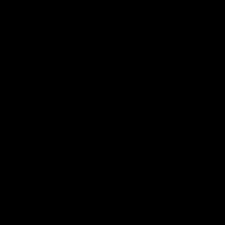
\includegraphics[width=22cm, height=15cm]{black.png}};
         \node {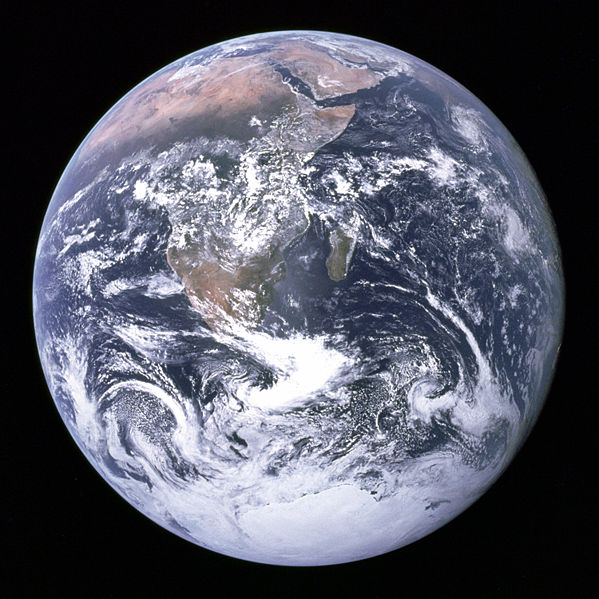
\includegraphics[scale=1]{terre.jpg}};
\end{pgfonlayer}  

\pgfmathsetmacro{\s}{0.15}

  %\foreach \i in {-2.5,-1.5,...,2.5}
  %    \foreach \j in {-2,-1,...,2.}
        %\foreach \k in {-2,-.5,...,2.}
  %          \draw[->, color=red, line width=0.5pt] 
              %(\i, \j+0.2, \k) -- (\i+ 0.5,  \j+0.3, \k  - 0.4);
  %            (\i, \j) -- (\i+ 0.4,  \j+0.2);

    %\draw[->, color=red, line width=1pt] (2, 3) -- (2+ 0.4,  3+0.2);
    %\draw[->, color=red, line width=0.7pt] (1, 3) -- (1+ 0.4,  3+0.2);
    %\draw[->, color=red, line width=0.3pt] (-1, 3) -- (-1+ 0.4,  3+0.2);
    %\draw[->, color=red, line width=0.5pt] (0, 3) -- (0+ 0.4,  3+0.2);
    %\draw [ball color=cyan!30!blue, opacity=0.7,very thin] (0.5,0.5,0.75) circle (1) ;

    \foreach \i in {-10,-9.9,...,10}
        \pgfmathsetmacro{\line}{2*rand^2}
        \pgfmathsetmacro{\size}{2}
        \draw[-latex, color=red, line width=\line pt] (rand*10, rand*7) ++ (0,0) --++ (\size*0.4,\size*0.2);


\pgfmathsetmacro{\s}{2}


  % draw the cube
  %\draw[white, very thin, opacity=0.5] (-\s,\s,\s)--(\s,\s,\s);
  %\draw[white, very thin, opacity=0.5] (-\s,\s,-\s)--(\s,\s,-\s);
  %\draw[white, very thin, opacity=0.5] (-\s,\s,\s)--(-\s,\s,-\s);
  %\draw[white, very thin, opacity=0.5] (\s,\s,\s)--(\s,\s,-\s);

  %\draw[white, very thin, opacity=0.5] (-\s,-\s,\s)--(\s,-\s,\s);
  %\draw[white, very thin, opacity=0.5] (-\s,-\s,-\s)--(\s,-\s,-\s);
  %\draw[white, very thin, opacity=0.5] (-\s,-\s,\s)--(-\s,-\s,-\s);
  %\draw[white, very thin, opacity=0.5] (\s,-\s,\s)--(\s,-\s,-\s);

  %\draw[white, very thin, opacity=0.5] (-\s,\s,\s)--(-\s,-\s,\s);
  %\draw[white, very thin, opacity=0.5] (-\s,\s,-\s)--(-\s,-\s,-\s);
  %\draw[white, very thin, opacity=0.5] (-\s,\s,\s)--(-\s,-\s,\s);
  %\draw[white, very thin, opacity=0.5] (\s,\s,\s)--(\s,-\s,\s);
  %\draw[white, very thin, opacity=0.5] (\s,\s,-\s)--(\s,-\s,-\s);

  \draw[blue];


\end{tikzpicture}

\end{document}
